The LLVM project started in 2000 by Chris Lattner, as a research project at the University of Illinois with the goal of providing a modern, Static Single Assignment (SSA)-based compilation strategy capable of supporting both static and dynamic compilation of arbitrary programming languages. It was first released in 2003, although the project has grown rapidly since then. It has become popular amongst major companies, e.g. Google, Apple and Sony, for its powerful multi-stage compilation strategy and outstanding extendibility. LLVM is a collection of modular and reusable compiler and toolchain technologies. Generally, LLVM follows a 3-phase design, which is divided up in a frontend, a code independent optimizer and a backend, illustrated in Figure \ref{fig:3phase_design}.

\begin{figure}[H]
\centering
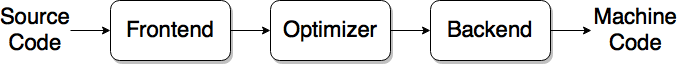
\includegraphics[width=.7\textwidth]{figures/3phase_design}
\caption{3-phase design: frontend, optimizer and backend.}
\label{fig:3phase_design}
\end{figure}

%Reorder list: [IR, Lexical analysis, Syntax analysis, ]
\textbf{The frontend} is responsible for translating code of an arbitrary language into LLVM's Intermediate Representation (IR) code. The LLVM instruction set represents a virtual architecture that captures the key operations of ordinary processors, but avoids machine specific constraints such as physical registers. Instead, it has an infinite amount of virtual registers in SSA form, which means that each virtual register is assigned only once and each use of a variable is dominated by that variable's definition. This simplifies the dataflow optimizations because only a single definition can reach a particular use of a value, and finding that definition is trivial \cite{llvm_strategy}.
%frontend talk, straight from the Dragon Book plz.
%introduce parser and lexical analysis and that it is kept in an AST, which will be translated as a final step to IR.
%Perhaps an example?
%TODO: rewrite first sentence in my own words.
As the first phase of a compiler, the main task of the lexical analyzer is to read the input characters of the source program, group them into luxemes, and produce as output a sequence of tokens. These tokens are used by the parser for syntax analysis, where we verify that the sequence of tokens can be reconstructed according to the syntax of the input language. The parser should report any syntax errors during this process and should be able to recover in order to continue processing the rest of the program. The parser constructs a parse tree, and the semantic analyzer uses this parse tree to check for consistency with the language definition. Type checking is also done during this stage, and the information is kept in the syntax tree. The result of these phases is an Abstract Synctax Tree (AST) of the program, which can be translated into three-address IR code. %We will discuss LLVM's IR in more detail in Chapter \ref{sec:ir}

\textbf{The optimizer} contains a collections of analysis and semantic-preserving transformations that can be used to optimize IR code. One of the advantages of LLVM is that when you build a new backend for any given processor architecture you immediately have access to all of these optimizations. Below we give some of these optimizations that are explained more detailed in literature \cite[Chapter~9]{dragon_book}.%TODO: provide chapter in cite.
\begin{itemize}
\item \emph{Constant propagation} computes for each point and each variable in the program, whether that variable has a unique constant value at that point. This can then be used to replace variable references with constant values.
\item \emph{Constant folding} recognizes and evaluates constant expressions at compile time rather than runtime. For example, `$add\ 1+2$' can be replaced by `$3$'. Statements like `$add\ 1+2$' can be introduced by other optimizations, e.g. constant propagation. 
\item \emph{Common sub-expression elimination} recognizes that the same expressions appears in more than one place, and that performance can be improved by transforming the code such that the expression appears in one only place.
\item \emph{Copy propagation} replaces each target of a copy statement with that of the copied value. For example, if we have a copy statement, $x = y$. Then the uses of $x$ can be replaced by $y$. Some optimizations require that this optimizations is performed afterwards to cleanup, e.g. common sub-expression elimination requires this pass to run afterwards. 
\item \emph{Dead code elimination} removes code that do not affect the programs results. This avoids executing irrelevant operations and reduces the code size of a program.  
\item \emph{Loop invariant code motion} aims at moving code that is independent of the loop iteration out of the loop body. It does this by moving the loop independent statement above the loop, saving it in a temporary variable, and use it in each iteration of the loop. Now the loop independent statement is computed only once instead of every iteration. 
\item \emph{Function inlining} verifies whether inlining functions in its callees gives a performance benefit. If doing this would give performance benefit, it replaces the call of the function with the function body. This optimization often is useful for small functions because it reduces the overhead that is introduced when a function call is made, e.g. storing frame pointer, storing function parameters and jump in code to where the function is defined.     
\end{itemize}

\begin{figure}[b!]
\centering
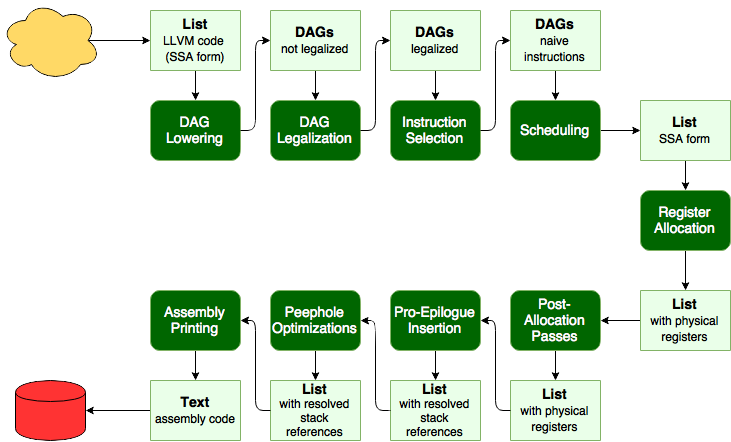
\includegraphics[width=\textwidth]{figures/code_generation_sequence}
\caption{Code generation sequence, from LLVM code to assembly code.}
\label{fig:code_generation}
\end{figure}

%TODO: apply following namings: Instruction, Machine instruction, scheduled instruction in SSA form, schedule instruction not in SSA form.
\textbf{The backend} translates, according to a processor architecture, IR code to a target specific assembly language. It does this by going through a sequence of code generation stages, illustrated in Figure \ref{fig:code_generation}. The rectangular boxes indicate the data structure that is used by, and produced by a given stage, and the name of each stage is denoted in a rectangular box with rounded corners. During this process, first the IR code is lowered to a Directed Acyclic Graph (DAG) in which each node represents one instruction. However, for some architectures, not all data types and instructions are supported. For this reason, the DAG is legalized to something that is supported by the target architecture. Instruction selection maps each of the nodes into machine nodes, by matching patterns. %After that, the instruction selector maps the pattern of LLVM code into the target machine code and builds a new DAG whose nodes represents the target instructions.
Then we have a DAG consisting of only target specific machine instructions, in SSA form. Having naive machine instruction, the next step is to schedule them. We schedule the machine instructions according to the resource information of the target processor, and assign each instruction to a specific cycle. 
%We will discuss scheduling in more detail in Chapter \ref{sec:scheduling}. 
Now the instructions are represented in a list rather than a DAG, but still in SSA form. The Register Allocator (RA) then assigns physical registers to each of the virtual registers, now the list is not in SSA form. 
%We will discuss RA in more detail in Chapter \ref{sec:register_allocation}. 
The post-allocation pass can improve the schedule, taking the physical registers and register pressure, that is known at this point, into account. After that, some epilogue and prologue code might need to be inserted, e.g. saving/restoring the caller/callee registers and reserving/destroying of the function's stack frame. The peephole optimizations are target specific improvements to the schedule that has been constructed. These optimizations deal with very specific optimizations that can only be done at the end of the process. At last, the assembly printer, prints the assembly code.
%backend talk -> huuge



%\subsection{Instruction Scheduling}\label{sec:scheduling}
%After instruction selection, the program is represented in SSA form as a DAG. Each instruction is represented as a $MachineSDNode$ in a $MachineBasicBlock$. After scheduling has been performed, each instructions now is represented as a $MachineInstr$. 



%ach instruction is scheduleDuring instruction schdduling, each $MachineBasicBlock$ is scheduled by the scheduler and transformed into a $MachineInstr$. After this phase, instructions are represented as $MachineInstr$.

%\subsection{Register Allocation}\label{sec:register_allocation}
%Register allocation is executed during the code generation phase and consists of finding a mapping of a program with an unlimited number of virtual registers to a program with a limited number of physical registers.
%Examples, machine instrs on the left in SSA form, on the right with proper registers next to it.
%Introduce at least 

\subsection{Scheduling and RA}
TODO: exlain phase ordering between scheduling and RA, from ref \cite[Chapter~10.2.4]{dragon_book}.

Introduce terms spilling, register pressure, and use this reference \cite{ra}.




%Additional ref. 
%




